\section{Identification}\label{sec:basics_identificationn}
As we mentioned, the use of a proximity operator to handle the nonsmooth part $r$ plays a prominent role, as it typically enforces some ``sparsity'' structure on the iterates and eventually on optimal solutions, see e.g.,\;\cite{vaiter2015model}. For instance, the popular $\ell_1$-norm regularization ($r=\|\cdot\|_1$) promotes optimal solutions with a few nonzero elements, and its associated proximity operator (called soft-thresholding, see\;\cite{donoho1995noising}) zeroes entries along the iterations. This is an example of \emph{identification}: in general, the iterates produced by proximal algorithms eventually reach some sparsity pattern close to the one of the optimal solution. For $\ell_1$-norm regularization, this means that after a finite but unknown number of iterations, the algorithm ``identifies'' the final set of non-zero variables. This active-set identification property is typical of constrained convex optimization (see e.g.\;\cite{wright1993identifiable}) and nonsmooth optimization (see e.g.\;\cite{hare2004identifying}).

The study of identification dates back at least to \cite{bertsekas1976goldstein} who showed that the projected gradient method identifies a sparsity pattern when using non-negative constraints. Such identification has been extensively studied in more general settings; we refer to \cite{burke1988identification}, \cite{lewis2002active}, \cite{drusvyatskiy2014optimality} or the recent \cite{lewis2018partial}, among other references.
Recent works on this topic include: i) extended identification for a class of functions showing strong primal-dual structure, including TV-regularization and nuclear norm \cite{fadili2018sensitivity}; ii) identification properties of various randomized algorithms, such as coordinate descent \cite{wright2012accelerated} and stochastic methods \cite{poon2018local,fadili2018model,sun2019we}.

The knowledge of the optimal substructure would allow to reduce the optimization problem in this substructure and solve a lower dimension problem. While identification can be guaranteed in special cases  (e.g.\;using duality\;for $\ell_1$-regularized least-squares \cite{ogawa2013safe, fercoq2015mind}), 
%dimension reduction methods have proven to be highly profitable it is usually unknown beforehand, and proximal algorithms can be exploited to obtain approximations of this substructure.
%  
After some substructure identification, one could switch to a more sophisticated method, e.g.\,updating parameters of first-order methods (\cite{liang2017activity}).
% or using restricted Newton's steps (XXX U-newton claudia, daniilidis-malick).
Again, since the final identification moment is not known, numerically exploiting identification to accelerate the convergence of first-order methods has to be done with great care.

In this section, we provide a general identification result for proximal algorithms useful for our developments, using the notion of sparsity vector.

\begin{definition}[Sparsity vector]\label{def:sparsity}
Let $\M= \{ \M_1,\ldots,\M_m\}$ be a family of subspaces of $\mathbb{R}^n$ with $m$ elements. We define the {sparsity vector} on $\M$ for point $x\in\mathbb{R}^n$ as the $\{0,1\}$-valued\footnote{For two vectors $a,b\in\{0,1\}^m$, we use the following notation and terminology: (1) if  $a_{[i]} \leq b_{[i]}$ for all $i=1,..,m$, we say that $b$ is greater than $a$, noted $a\leq b$; and (2) we define the union $c = a\cup b$ as $c_{[i]} = 1 $ if $a_{[i]} = 1$ or $b_{[i]}=1$ and $0$ elsewhere.} vector  $\S(x)\in \{0,1\}^m$ verifying
\begin{align}\label{eq:strata}
    \left( \S(x) \right)_{[i]} = 0 \quad\text{ if } x \in \M_i \text{ and } 1 \text{ elsewhere}.
\end{align}
%The sparsity measure (with respect to a given $\M$) of a point $x$ is defined by the number of subspaces containing $x$, i.e.\;$s(x)=\|\S(x)\|_1$. We will use this measure in our numerical experiments.
\end{definition}

An identification result is a theorem stating that the iterates of the considered algorithm eventually belong to some -- but not all -- subspaces in $\M$. We formulate such a result of almost surely converging proximal-based algorithms as follows. This very simple result is inspired by the extended identification result of \cite{fadili2018sensitivity} (but does not rely on strong primal-dual structures as presented in \cite{fadili2018sensitivity}).

\begin{theorem}[Enlarged identification]\label{th:identification}
Let $(u^k)$ be an $\mathbb{R}^n$-valued sequence converging almost surely to $u^\star$ and define sequence $(x^k)$ as $x^k = \prox_{\gamma g}(u^k)$ and  $x^\star =  \prox_{\gamma g}(u^\star)$. Then $(x^k)$ identifies some subspaces with probability one; more precisely for any $\varepsilon>0$, with probability one, after some finite time,
\begin{equation}\label{eq:identification_result}
     \S(x^\star) ~\leq~ \S(x^k) ~\leq\!\!\bigcup_{u\in\mathcal{B}(u^\star,\varepsilon)} \!\S(\prox_{\gamma g}(u)).
\end{equation}
\end{theorem}
\begin{proof}[Proof of Theorem \ref{th:identification}]
The proof is divided between the two inequalities. We start with the right inequality. As $u^k \to u^\star$ almost surely, for any $\varepsilon>0$, $u^k$ will belong to a ball centered around $u^\star$ of radius $\varepsilon$ in finite time with probability one. Then, trivially, it will belong to a subspace if all points in this ball belong to it, which corresponds to the second inequality.

Let us turn now to the proof of the left inequality.  Consider the sets to which $x^\star$ belongs i.e. $\M^\star = \{ \M_i\in\M : x^\star \in \M_i \}$; as $\M$ is a family of subspaces, there exists a ball of radius $\varepsilon'>0$ around $x^\star$ such that no point $x$ in it belong to {more} subspaces than $x^\star$ i.e. $x \notin \M \setminus \M^\star$. As $x^k \to x^\star $ almost surely, it will reach this ball in finite time with probability one and thus belong to fewer subspaces than $x^\star$.
\end{proof}

Let us present a couple of important examples of the regularizers that enforce sparsity of the final solution (\cite{argyriou2013sparsity}, \cite{jenatton2011structured}, \cite{zhao2006grouped}). The most common types of sparsity are (block) coordinate one, when there are only a few non-zero (blocks of) coordinates and variation one when there are few continuous blocks of coordinates such that the coordinates inside of each are the same.

\begin{example}[$\ell_{1,2}$ regularizer]\label{ex:intro_coordinate_strata}
    It is known that if $r$ is $\ell_{1,2}$ regularizer induced by non-overlapping partition $\mathcal{B}$ reads
    \begin{equation}\label{eq:l12}
         r(x) = \sum\limits_{B\in\mathcal{B}}\|x^B\|_2, 
    \end{equation}
    where $x^B$ is the restriction of $x$ to the entries indexed by block $B$, it enforces block sparsity i.e. it derives all the coefficients in one block to zero together (regularizer $\ell_1$ is a particular case of $\ell_{1,2}$ so it leads to coordinate sparsity).
    
    In this case the support of the optimal point $x^\star$ will be small, where 
    \begin{equation}\label{eq:supp}
        \supp(x) \stackrel{\triangle}{=}\left\{i\in [1,n]\,| x_{[i]} \neq 0 \right\}.
    \end{equation}
    Let us specify a family $\M$ for the case of $\ell_{1,2}$ regularizer (or even ones that enforce (block) coordinate sparsity.)
    
    Let us define collection $\M = \{\M_i\}_{1\leq i\leq d}$ as the set of all subspaces $\M_i$ with fixed support i.e. $\supp(x) = \supp(y)$ for all $x,y\in \M_i$. In case of this collection, identification result \eqref{eq:identification_result} can be reformulated as
    \begin{equation}\label{eq:ident_l1}
        \supp(x^\star) \subseteq \supp(x^k) \subseteq \bigcup_{u\in\mathcal{B}(u^\star,\varepsilon)} \supp(\prox_{\gamma r}(u)).
    \end{equation}
    
    To prove this it is enough to show that
    \begin{equation}\label{eq:s_to_supp}
        \S(x)\leq\S(y) \iff \supp(x)\subseteq\supp(y).
    \end{equation}
    
    It follows from the definition that if $\M_i\subseteq \M_j$ then $(\S(x))_{[i]}\leq(\S(x))_{[j]}$ for any $x$. Using this fact let us prove this remark.
    
    $(\Rightarrow)$ Let  $\S(x)\leq\S(y)$ then for all $i = 1,\dots,d$ it is true that $(\S(x))_{[i]}\leq(\S(y))_{[i]}$. Choosing $j$ such that $\supp(\M_j) = \supp(y)$ we have $(\S(x))_{[j]}= 0$ that means $\supp(x)\subseteq\supp(y)$.
    
    $(\Leftarrow)$ $(\S(y))_{[i]} = 0$ if $\supp(y)\subseteq\supp(\M_i)$. In this case, $\supp(x)\subseteq\supp(y)\subseteq\supp(\M_i)$ that implies $(\S(x))_{[i]} = 0 = (\S(y))_{[i]}$. On the other hand, if $(\S(y))_{[i]} = 1$ then $(\S(x))_{[i]}\leq(\S(y))_{[i]}$ that finishes the proof of \eqref{eq:s_to_supp}.
\end{example}

The identification result in case of regularizer $r$ that enforce (block) coordinate sparsity case can be clearly seen in the example of proximal gradient descent for $\ell_1$ regularized problems.

%It also can be seen that before identification moment, some coordinates from the support of optimal points were outside of the current's point support even if they were before.

\begin{figure}[H]
\centering

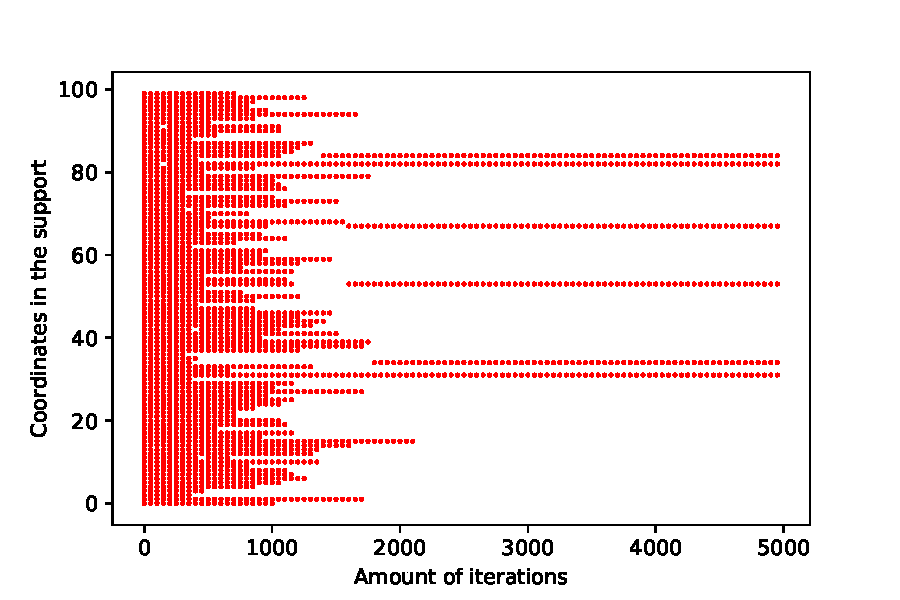
\includegraphics{basics_2/l1_supp.pdf}
\caption{$\ell_1$ identification}
\label{fig:l1supp}
\end{figure}

% \input{Article/l1_identification.tex}

In Figure~\ref{fig:l1supp} we can see how support changes during proximal gradient descent for LASSO problem 
$$
\min~\frac12\|Ax-b\|_2^2 + \lambda_1\|x\|_1
$$
for random generated matrix $A\in\mathbb{R}^{100\times100}$ and vector $b\in\mathbb{R}^{100}$ and hyperparameter $\lambda_1$ chosen to reach $6\%$ of density (amount of non-zero coordinates) of the final solution.
Starting from $500^{\text{th}}$ iteration, the support of iterates begins to change and becomes stable after $2000$.


Another important example of sparsity inducing regularizer is $1$-d $\mathbf{TV}$ regularizer.
\begin{example}[$\mathbf{TV}$ regularizer]\label{ex:intro_jump_strata}
It is known that if $r$ is $1$-d $\mathbf{TV}$ regularizer
\begin{equation}\label{eq:tvreg}
    r(x) = \sum\limits_{i=1}^{n-1}|x_{[i]} - x_{[i+1]}|
\end{equation}
it enforces variation sparsity.    

In this case the amount of jumps (blocks) in optimal solution $x^\star$ will be small, where
\begin{equation}
\jumps(x)\stackrel{\triangle}{=} \left\{i\in [2,n]\,| x_{[i]} \neq x_{[i-1]} \right\}.    
\end{equation}

Let us define collection $\M = \{\M_i\}_{1\leq i\leq d}$ as the set of all subspaces $\M_i$ with the fixed block structure i.e. $\jumps(x) = \jumps(y)$ for all $x,y\in \M_i$. In case of this collection, identification result \eqref{eq:identification_result} can be reformulated as
\begin{equation}\label{eq:ident_tv}
    \jumps(x^\star) \subseteq \jumps(x^k) \subseteq \bigcup_{u\in\mathcal{B}(u^\star,\varepsilon)} \jumps(\prox_{\gamma r}(u)).
\end{equation}

To prove this it is enough to show that
\begin{equation}\label{eq:s_to_jumps}
    \S(x)\leq\S(y) \iff \jumps(x)\subseteq\jumps(y),
\end{equation}
which proves exactly the same way as \eqref{eq:s_to_supp}.

\end{example}


% This result yields immediately that the iterates of the subspace descent method presented in Section~\ref{sec:algo} will reach some ``structure'': they will belong to some of the subspaces in $\M$ after some finite time with probability one, and these subspaces are sandwiched between the two extremes families of subspaces controlled by the pair $(x^\star, u^\star)$. 
The Theorem \ref{th:identification} explains that iterates of any converging proximal algorithm will eventually be sandwiched between two extremes families of subspaces controlled by the pair $(x^\star, u^\star)$.